\section{Finite Element Spaces, Meshes and Indexing}

To implement the Finite Element Method, functions are needed to map mesh vertices to elements and vice-versa.
In our implementation, this is implemented in the \texttt{FiniteElementSpace} class. It is also the base
class for the \texttt{LagrangeSpace} class that implements Lagrangian finite elements.
The \texttt{FiniteElementSpace} class is an abstract class that implements the mesh helper functions and also declares pure virtual member
functions for degree-of-freedom, reference element shape function evaluations and assembly functions.

\subsection{Mesh vertex and element index mapping}

At this time, IPPL implements only structured, rectilinear grid meshes.
In FEM, each mesh cell is assigned an element. The elements are indexed starting from zero (\texttt{C++} indexing)
in this implementation.

To define the position of a vertex in the structured rectilinear grid mesh,
we define a vector that has $N$ entries for an $N$ dimensional mesh with each entry representing
the position of a mesh cell in the $n$-th dimension.
In the implementation, the type alias for this vector is called \texttt{NDIndex},
following the naming convention from IPPL.

For example, in figure \ref{fig:mesh} the \texttt{NDIndex} of vertex $13$ would be $(3, 2)$.
The element \texttt{NDIndex} of $(3,1)$ corresponds to the element with index $7$.

Figure \ref{fig:mesh} illustrates the mesh vertex indexing (black) and element indexing (red).
Each vertex index is associated with the vertex \texttt{NDIndex},
as well as each element associated with the element \texttt{NDIndex}.

\begin{figure}[h]
    \centering
    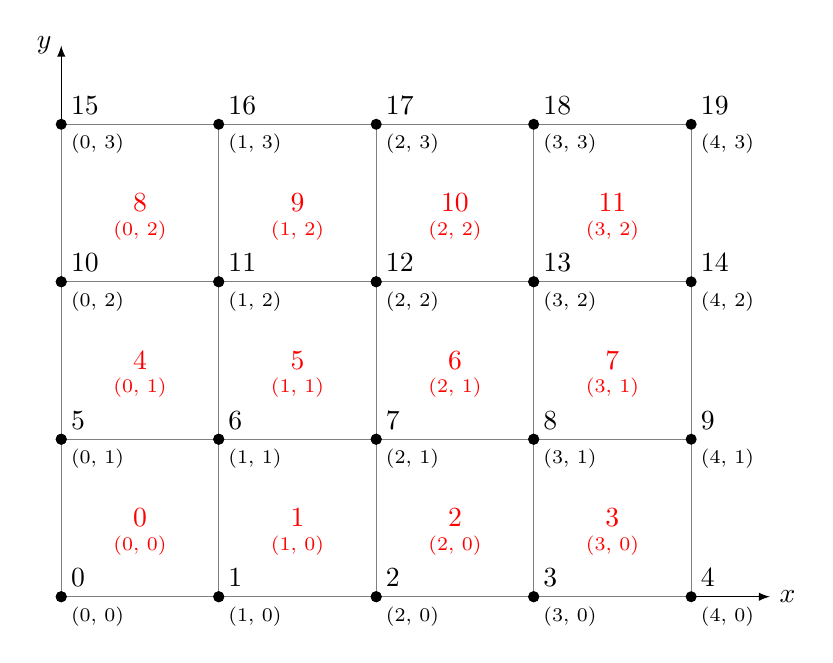
\begin{tikzpicture}
        \draw[-latex] (0,0) -- (9,0) node[right] {$x$};
        \draw[-latex] (0,0) -- (0,7) node[left] {$y$};

        % Draw grid over highlighted cells
        \draw[step=2cm,gray,very thin] (0,0) grid (8,6);

        % Mesh vertices
        \foreach \x in {0,1,2,3,4} {
                \foreach \y in {0,1,2,3} {
                        \fill (2*\x,2*\y) circle (2pt);
                        \pgfmathtruncatemacro\index{5*\y + \x}
                        \node[black, anchor=south west] at (2*\x,2*\y) {\index};
                        \node[black, font=\scriptsize, anchor=north west] at (2*\x,2*\y) {(\x, \y)};
                    }
            }

        % Elements
        \foreach \x in {0,1,2,3} {
                \foreach \y in {0,1,2} {
                        \fill (2*\x,2*\y) circle (2pt);
                        \pgfmathtruncatemacro\index{4*\y + \x}
                        \node[red] at (2*\x+1, 2*\y+1) {\index};
                        \node[red, font=\scriptsize, anchor=north] at (2*\x+1, 2*\y+0.9) {(\x, \y)};
                    }
            }
    \end{tikzpicture}

    \caption{Illustration of mesh vertex indexing and element indexing.}
    \label{fig:mesh}
\end{figure}

\subsection{The FiniteElementSpace Class}

The \texttt{FiniteElementSpace} class takes in template arguments for the floating point type \texttt{T},
the dimension \texttt{Dim} and the number of degrees of freedom on a reference element \texttt{NumElementDOFs}
the quadrature rule type \texttt{QuadratureType} and the two types for the left-hand-side IPPL \texttt{Field} and the right-hand-side IPPL \texttt{Field}.

This class declares additional pure virtual member functions in the header file, that child classes
need to define. These functions are for degrees of freedom, reference element shape functions evaluations and assembly operations and they
will be introduced in section \ref{sec:lagrange_class}.

